\documentclass[]{nrel}

\usepackage{lipsum}

% -----------------------------------
% DOCUMENT PROPERTIES
% -----------------------------------
\title{NREL Report---Full Guidance Document}

\author{Nicholas Hamilton}
\author{Chioke Harris}
\affil{National Renewable Energy Laboratory}
\author{Author Four}
\affil{Another affiliation}
\author{Author Five}
\affil{A third affiliation}


\fancypagestyle{plain}{}
\addbibresource{files/refs.bib}
\setcounter{tocdepth}{2}

% -------------------------------------
% DOCUMENT STARTS HERE
% -------------------------------------
\begin{document}

\frontmatter
\chapter{Executive Summary}
This document is a guide to writing documents for publication by NREL using the LaTeX document preparation system. LaTeX is not WYSIWYG and has different reviewing and editing tools compared to typical word processing software. For this reason special care has to be taken when preparing NREL documents in LaTeX.


This document serves both as a guide to implementing NREL's style and formatting guidelines in LaTeX, and as a template. This document is intended for people with some familiarity with LaTeX.

\chapter{Acknowledgments}
Updates to this template are made by Nicholas Hamilton with support and style guidance from  Sheri Anstedt, Kimberly Austin, Deanna Cooke, and Chioke Harris.

The original document and the NREL LaTeX class file were developed by staff at the National Wind Technology Center, including Andrew Platt, Andrew Clifton, Andrew Ning, Mike Lawson, and Paul Fleming. Alexsandra Lemke provided support relating to NREL communications. A first demonstration of an NREL class file was created by Chuck Booten from NREL's Electricity, Resources, and Building Systems Integration group, which inspired this effort. The class file and this template were developed as part of work on several NREL reports, journal articles, and conference publications.

We thank members of the TeX -- LaTeX StackExchange site for useful suggestions concerning LaTeX and typography \citep{texstackexchange}.
This report was typeset using the LaTeX typesetting system originally developed by Leslie Lamport, based on TeX created by Donald Knuth. It was revised in 2014 by A. Clifton, A. Platt, M. Dennis, P. Fleming, and M. Lawson. The class file and examples were revised again in 2021 by N. Hamilton.

%%%%%%%%%%%%%%%%%%%%%%%%%%% 
\chapter{List of Acronyms} %<--------- Uncomment this section if adding acronyms
\begin{acronym}[ICANN]
    \acro  {DOE}  {Department of Energy}
    \acro  {NREL}  {National Renewable Energy Laboratory}
\end{acronym}

\mainmatter
\tableofcontents
\listoffigures
\listoftables


\chapter{Dummy chapter}
\section{Creating Content}
\subsection{Front, main, and back matter}
NREL's convention is to have Roman numerals in the front matter, and then arabic numerals in the main matter of the document (after the tables of contents, figures and tables). Tables and figures in the front matter are also numbered differently (Table A, B, C, ...) than in the main matter (Table 1, 2, 3, ...).

This change in page and float numbering is implemented using the \verb+\frontmatter+, \verb+\mainmatter+, and \verb+\backmatter+ commands at the start of these sections of the document:

\begin{lstlisting}
\begin{document}

\maketitle
\frontmatter
...
\tableofcontents
\clearpage
\listoffigures
\listoftables
\mainmatter
...
\backmatter
\end{document}
\end{lstlisting}

\section{Creating a file structure}
\label{sec:FileStructure}
Your main file should be called \emph{main.tex}. This helps editors and coauthors identify where to start. Then, use \texttt{input} to import other files into your main file at compilation.

For example, each of the chapters in this report is in separate files, called \emph{WhatIsLatex} (Chapter 1), \emph{NRELRequirements.tex} (Chapter 2), \emph{LatexAtNREL.tex} (Chapter 3), and so-on. In the example available on Github, they are stored in the \emph{files} directory. \emph{main.tex} then looks like this:

\begin{lstlisting}
...
\begin{document}
% content
\chapter{What is LaTeX?}
LaTeX is a mark-up language that describes how a document should be prepared.

Three things are needed to make a LaTeX document:
\begin{enumerate}
\item A source document, usually with extension \emph{.tex}
\item Some packages and classes that help turn what's in the source document into something helpful
\item A compiler, also referred to as a working LaTeX installation.
\end{enumerate}

At first glance the source document looks like a programming language, and that's because it is: LaTeX is not WYSIWYG, like many of the document preparation tools in common use today. A good analogy to LaTeX is html code, which can be read in any text editor but is rendered by web browsers into a finished product.

\section{Printed Resources}
Several excellent LaTeX references exist and may be found useful by some users. Examples include those by \citet{Knuth_1984_a} and \citet{Lamport_1986_a}.

\section{Online Resources}
The wikibook at \href{http://en.wikibooks.org/wiki/LaTeX}{http://en.wikibooks.org/wiki/LaTeX} is an excellent resource. There are also several internet forums such as \href{tex.stackexchange.com}{tex.stackexchange.com} that may be useful.

Documentation for the packages used in the nrel.cls file (Section \ref{sec:nrelcls}) can be found at \href{ctan.org}{ctan.org}.

\input{files/NRELRequirements}
\input{files/LatexAtNREL}
...
\end{lstlisting}

\section{Best practice in writing a document in LaTeX}
\begin{description}
  \item[Create a structure before you get too far.] Authors will find it easier to write documents and make changes if they separate the content of the document from the structure.
        \begin{enumerate}
          \item Each new LaTeX document should be placed in it's own directory.
          \item Create a main LaTeX file that just contains the preamble, custom commands and uses \texttt{input} to call the content. See Section \ref{sec:FileStructure} for an example where each \texttt{chapter} is contained in its own file. In an article, each \texttt{section} could be contained in its own file.
          \item Keep the number of packages used to a minimum. If authors feel that something is desperately missing, they can contact the maintainers of the \emph{nrel.cls} file. Not all packages can be used as they lack compatibility.
        \end{enumerate}
  \item[Focus on content, not appearance.] Don't spend hours trying to adjust fonts, headers or spacing between lines.
        \begin{enumerate}
          \item The document produced should meet NREL's requirements if it is compiled using \emph{nrel.cls}.
          \item Don't throw in lots of \texttt{clearpage}s or other commands to push material around. LaTeX is designed to handle that.
          \item Resist the temptation to add or subtract space, change lengths or do other things to modify the layout.
          \item Write!
        \end{enumerate}
\end{description}

\section{Dummy section}
\lipsum[5-6]
\cite{aitken2014quantifying,argrow2017ncar}


\lipsum[9]
Advantages of \href{latex.nrel.gov}{latex.nrel.gov} include:
\begin{enumerate}
  \item No need to maintain a local version of LaTeX
  \item Everyone uses the same version of LaTeX
  \item Editors and reviewers can work in a user-friendly environment
  \item There is an always-on ``track changes'' feature
  \item Secure hosting of documents within the NREL domain
  \item Ability to download source documents for archiving
\end{enumerate}

\chapter{Another dummy chapter}
\lipsum[3]
\cite{wildmann2018coplanar,klein2015lable,jagdish2018validation} 
See note below for more information.\footnote{This is a just a footnote to have an example in the text. }

\begin{itemize}
  \item {Meteorological masts and in-situ point measurements}
        \begin{itemize}
          \item Sonic anemometers
          \item Pressure-temperature-humidity
        \end{itemize}
  \item Remote sensing
        \begin{itemize}
          \item Sodar and radar radio acoustic sounding system)
          \item Ka-band and X-band radar
          \item A diversity of lidars (e.g., ground-based, nacelle-mounted, scanners, profilers)
          \item Field-particle-image-velocimetry-type systems
          \item Satellite imaging
        \end{itemize}
  \item Other instruments
        \begin{itemize}
          \item Radiosondes and sounding systems (difficult with the Federal Aviation Administration; labor-intensive)
          \item Eddy covariance (surface flux stations) both upwind and throughout the wind plant
          \item Ceilometer for planetary boundary layer heights
          \item SCADA (performance/operational data, loads)
          \item Upwelling/downwelling radiation sensors
          \item Sensors for surface properties (e.g. soil moisture/temperature, surface albedo,…)
          \item Tethered lifting systems
          \item Airborne measurement systems and unmanned aerial vehicles
        \end{itemize}
  \item Other advice
        \begin{itemize}
          \item Plan for backup units, (re)calibration of instruments, maintenance/downtime, data formatting, and time synchronization.
        \end{itemize}
\end{itemize}



\chapter{Yet another dummy chapter}

\subsection{Citations}
\label{Sec:Bib}
Use \texttt{bibtex} to organize references and store them in a single file (e.g. \verb+/Documents/bibliography/bibliography.bib+). The bibliography will then contain entries with `keys' for each source, like \texttt{Lamport\_1986\_a}.

Authors can then insert citations to this key throughout their document, using different styles of citation. Citations are generated using the \texttt{biblatex} package, which also formats references in the correct style.  Ways to generate citations are described in the \texttt{biblatex} documentation, and include:
\begin{itemize}
  \item \verb+\cite{moriarty2020american}+ prints \cite{moriarty2020american}.
  \item \verb+\citep{moriarty2020american}+ prints \citep{moriarty2020american}.
  \item \verb+\citet{moriarty2020american}+ prints \citet{moriarty2020american}.
  \item A more complex case: \verb+\parentext{\citet{moriarty2020american} and \citep{fernando2019perdigao}}+ prints \parentext{\citet{moriarty2020american} and \citep{fernando2019perdigao}}
\end{itemize}

To cite URLs, use the 'misc' style. For example, the bibtex entry for \href{http://tex.stackexchange.com}{http://tex.stackexchange.com}\ \cite{texstackexchange} looks like this:

\begin{lstlisting}
@misc{texstackexchange,
	Author = {Anon.},
	Howpublished = {Accessed July 21, 2014: \url{http://tex.stackexchange.com}},
	Title = {\TeX -- LaTeX Stack Exchange},
	Year = {2014}}
\end{lstlisting}

This format will allow you to include the date on which a URL was accessed.

The citations should work with journal articles \citep{Clifton_2013_a}, books \citep{Knuth_1984_a, Lamport_1986_a, chicago}, technical reports \citep{TechReportTest}, and URLs \citep{texstackexchange}. Any unknown publication types will be formatted using the `misc' type.

\subsection{Including computer code}
The \texttt{listings} package has been loaded. Note: this does not work if the `Draft' document option is used.

To change the syntax highlighting use \verb+\lstset{language=[dialect]language,columns=fullflexible,keepspaces=true}+ before each listing where the language changes. For more details see the \texttt{lstlisting} documentation.

\subsection{NREL-style bibliographies}
NREL uses "Chicago A" style-references. The \emph{nrel.cls} file uses Biblatex to produce these references automatically.

To include a bibliography in the document give the bibliography file location in the preamble, and insert the bibliography at the appropriate location:

\begin{lstlisting}
% give the bibliography file location
\bibliography{files/bibliography.bib}
...
\begin{document}
...
% insert the bibliography into the document
\cleardoublepage
\label{sec:Bib}
\printbibliography
...
\end{document}
\end{lstlisting}


\begin{figure}[t!]
  \centering
  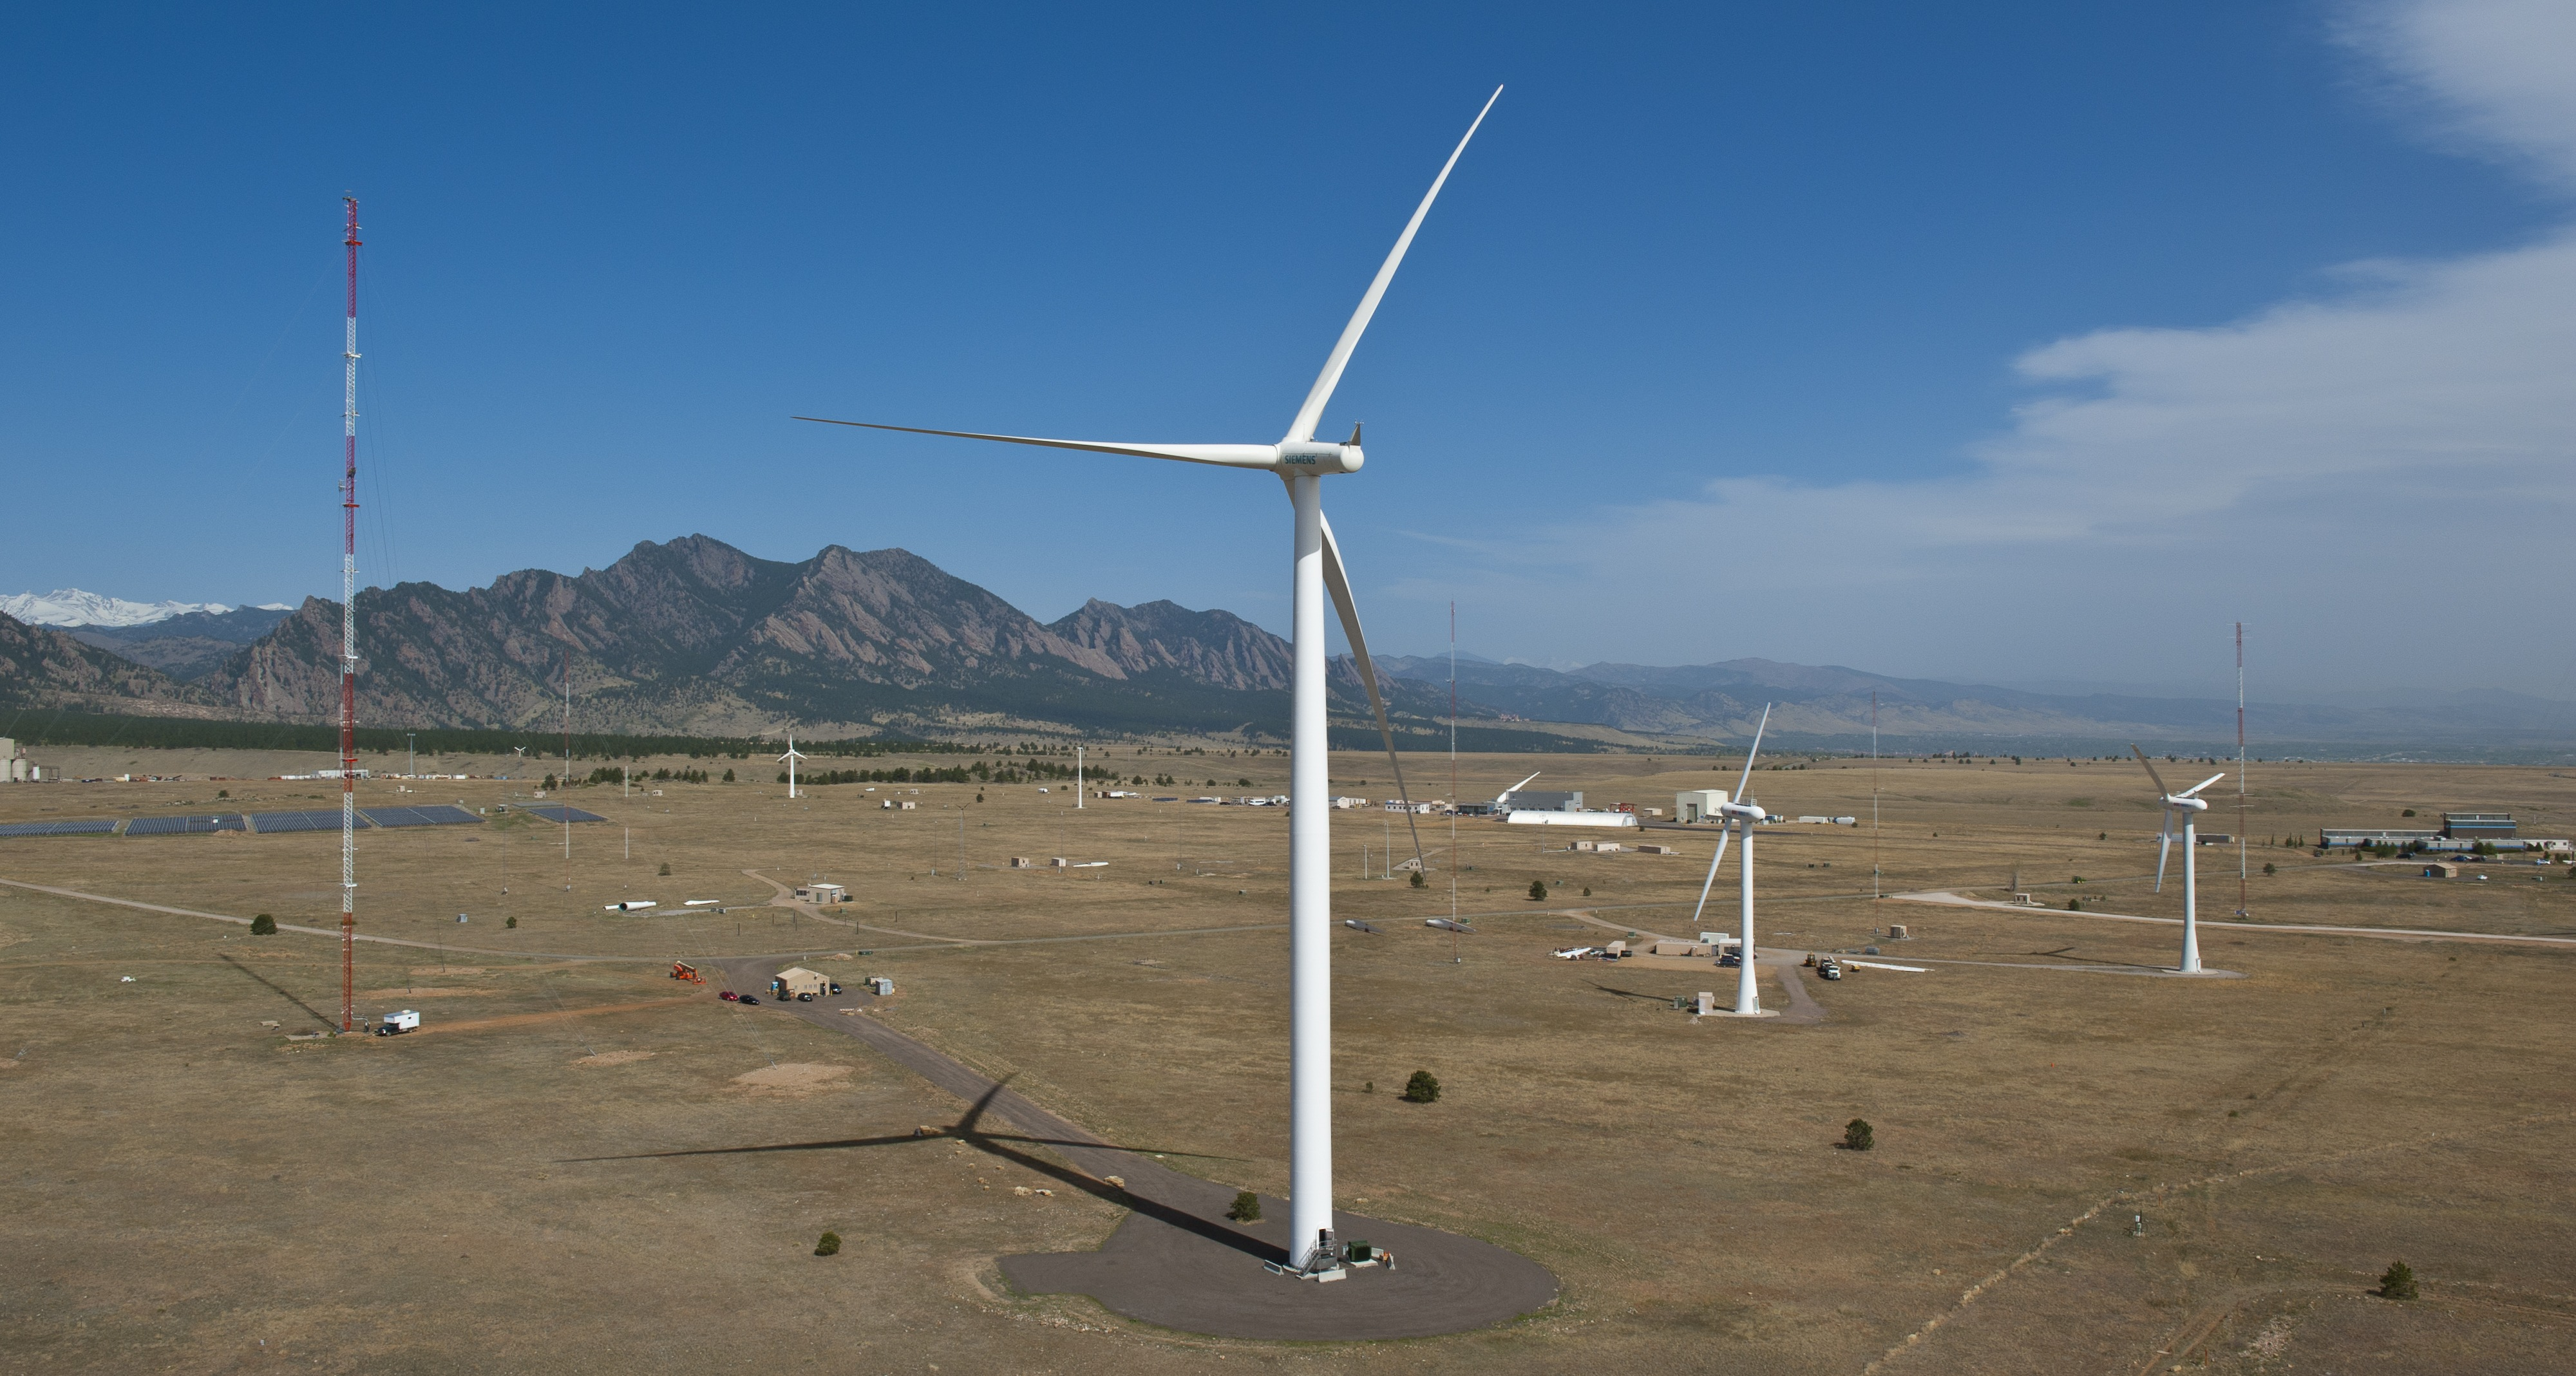
\includegraphics[width=\columnwidth]{files/20018.JPG}
  \caption{Very pretty picture \cite{Debnath2017,brock1995oklahoma,krishnamurthy2017offshore}}
  \label{fig:fig1}
\end{figure}

\lipsum[25-32]
\cite{fernando2019perdigao,banta2015,kasler2010wake}


\begin{figure}[h!]
  \centering
  \begin{subfigure}[b]{0.48\columnwidth}
    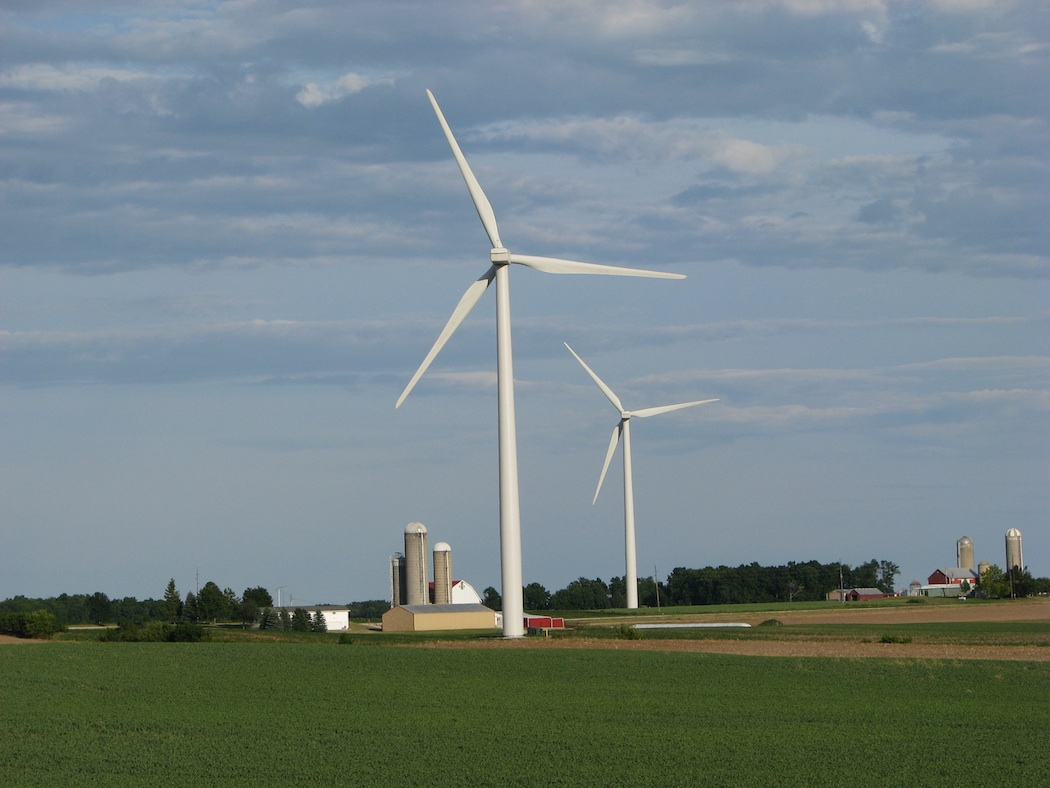
\includegraphics[width=\columnwidth]{files/21206.png}
    \caption{subfigure on the left}
    \label{fig:fig2a}
  \end{subfigure}
  \hfill
  \begin{subfigure}[b]{0.48\columnwidth}
    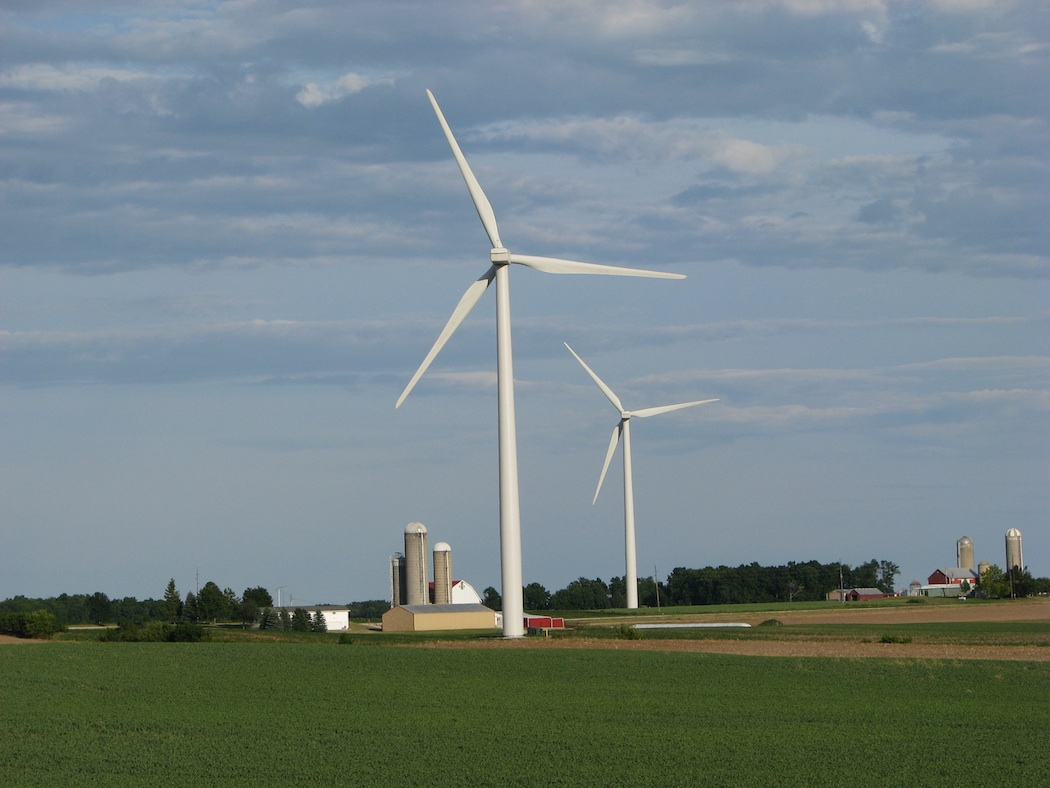
\includegraphics[width=\columnwidth]{files/21206.png}
    \caption{subfigure on the right}
    \label{fig:fig2b}
  \end{subfigure}
  \caption{Another pretty figure, this time with two pictures.}
  \label{fig:fig2}
\end{figure}


%%%%%%%%%%%%%%%%%%
% bibliography
\cleardoublepage
\label{sec:Bib}
\printbibliography[title={\LARGE References}]
\addcontentsline{toc}{chapter}{References}
% \nocite{*}

%%%%%%%%%%%%%%%%%%%%%%%%%%%%%%%%%%%%
\begin{appendices} %<--------- All chapters after this will be labeled as appendices

  \appchapter{Included packages}
  \lipsum[66]

  \begin{table}[!h]
    \centering
    \caption[Packages loaded by the NREL classes]{Packages loaded by the NREL classes.}
    \label{Tab:Packages}
    \begin{tabular}{llp{0.6\textwidth}}
      \toprule
      Package           & Options                & Functionality                                                                                    \\
      \midrule
      %accessibility & tagged & generates the document structure and tagging \\
      amsfonts, amssymb &                        & supplies AMS fonts, which are useful for mathematics                                             \\
      babel             & english                & activates language-appropriate hyphenation rules                                                 \\
      booktabs          &                        & improves the formatting of tables                                                                \\
      caption           &                        & required to generate captions for floats                                                         \\
      courier           &                        & changes fonts                                                                                    \\
      fontenc           & T1                     & enables direct typing of international characters                                                \\
      geometry          &                        & sets page size and margins                                                                       \\
      graphicx          &                        & graphics handling, including \emph{.eps} figures                                                 \\
      helvet            & scaled=0.83            & sets helvetica as the default sans-serif font, with correct scaling to match the serif font size \\
      hyphenat          &                        & improves spacing and breaking of hyphenated words                                                \\
      listings          &                        & enables the inclusion of high-quality computer code listings                                     \\
      mathptmx          &                        & changes fonts                                                                                    \\
      nag               &                        & checks that packages are up to date and looks for bad habits in LaTeX code.                      \\
      parskip           &                        & required for better spacing                                                                      \\
      pdfcomment        &                        & required for tool-tips. Also calls the \texttt{hyperref} package                                 \\
      setspace          &                        & required for better spacing                                                                      \\
      subcaption        &                        & provides the \texttt{subfigure} environment to produce sub figures                               \\
      tocloft           &                        & improved table of contents and list of files/tables in memoir documents                        \\
      tocbibind         & nottoc, notlot, notlof & Add bibliography/index/contents to Table of Contents in memoir documents                         \\
      todonotes         &                        & inline and margin to-do notes                                                                    \\
      xcolor            &                        & Driver-independent color extensions for LaTeX and pdfLaTeX                                       \\
      \bottomrule
    \end{tabular}
  \end{table}

  \appchapter{Supplemental Information}
  \lipsum{77-82}

  % \chapter{Even More Supplemental Information}
  % \label{app:B}

\end{appendices}
%%%%%%%%%%%%%%%%%%%%%%%%%%%%%%%%%%%%
\end{document}
